%% $Id: domaincoloring-doc.tex 979 2024-09-02 16:07:29Z herbert $
% 
\listfiles

\def\header{Complex Functions}

\DocumentMetadata{}
\documentclass[fontsize=11pt,english,BCOR=10mm,DIV=12,bibliography=totoc,parskip=false,headings=small,
    headinclude=false,footinclude=false,oneside]{pst-doc}
\listfiles

\usepackage{biblatex}
\addbibresource{\jobname.bib}

\usepackage{booktabs} % for examples
\usepackage{xltabular} % for examples
\usepackage{enumitem}
\setlist{noitemsep,nosep}

\usepackage{makeidx}
\makeindex

\usepackage{domaincoloring}
\let\DColFV\fileversion
\setDColkeys{force=false}% only for this documentation relevant

\usepackage{hvlogos} 

\usepackage{listings}
\lstset{columns=fixed,basicstyle=\ttfamily\small}

\def\bgImage{\hspace{-2cm}*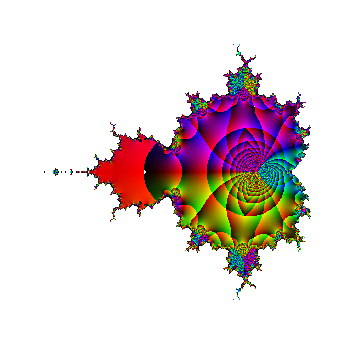
\includegraphics[width=14cm]{titleImg.png}}

\title{Domain Coloring of complex functions\\version \DColFV}
\author{Herbert Voß}
\begin{document}
\settitle
\tableofcontents


\section{Introduction}

This package works only with \texttt{lualatex} and the option \Loption{shell-escape}! 
It creates an intermediate external EPS-file, which is automatically converted with
\LFile{epstopdf}. The pdf is in the end imported by the macro \Lcs{includegraphics}.

\subsection{Loading the package}
The package \texttt{domaincoloring} creates acolored interpretation of the
domain of a complex function. The package itself has no options and should be loaded as
usual:

\begin{verbatim}
\usepackage{domaincoloring}
\end{verbatim}

The package needs the following Lua modules:

\begin{itemize}
\item \texttt{domaincoloring.lua}   the main module
\item \texttt{domaincoloring-complex-numbers.lua} for complex math operations
\item \texttt{domaincoloring-functions.lua}   for predefined complex functions
\end{itemize}

The function module has to be managed  by the user himself, if needed.



\subsection{Using the macro}

There is only one macro which does the external call of the Lua program \verb|domaincoloring.lua|.
This program creates the image which is then included into the document. The \LaTeX-run needs
the \verb|--shell-escape| option to allow the external run of the program to convert the created
eps-file into a pdf file, which is then included by the command \Lcs{includegraphics} into
the document.


\begin{verbatim}
\DomainColoring[options]{complex function in Lua notation}
\end{verbatim}

Every math function has to be preceeded by \texttt{cmath} if it has a complex argument.
The following complex functions are supported:

\begin{verbatim}
complex(re,im)         creates a complex number from real and imaginary components.
re(z)                  real part of z
im(z)                  imaginary part of z
arg(z)                 argument of z
abs(z)                 absolute value of z
sqrt(z)                z^0.5
pow(x,y)               x^y
exp(z)                 e^z
ln(z)                  e^? = z
log(b,z)               ln(z)/ln(b)
sin(z)
cos(z)
tan(z)
sinh(z)
cosh(z)
tanh(z)
asin(z)
acos(z)
atan(z)
atan2(y,x)
asinh(z)
acosh(z)
atanh(z)
polar(z)               returns r,phi = cmath.abs(z),cmath.arg(z)
rect(r,phi)            returns a complex number from polar = r*e^(i*phi)
diff(z)                returns re(z)^2-im(z)^2
zeta(z[,accuracy=1e4]) riemann zeta function
lintegrate(f,H,[L=0,n=sensible for H])
cx(string)             creates a complex number from a string (e.g. "1.1-i" -> 1.1+-1i)
cx(re,im)              same as complex(re,im)
\end{verbatim}

The default trigonometrical functions can be used without a preceeding \verb|math|: 

\begin{verbatim}
e=math.exp(1)
pi=math.pi
abs=math.abs
exp=math.exp
log=math.log
cos=math.cos
sin=math.sin
cosh=math.cosh
sinh=math.sinh
sqrt=math.sqrt
atan2=math.atan2
\end{verbatim}



\subsection{Options}

\noindent
\begin{xltabular}{\linewidth}{@{} >{\ttfamily}l l X @{}}\\\toprule
\emph{name} & \emph{value} &\emph{meaning}\\\midrule
\Lkeyword{domain} & {-2,2,-2,2} & the (re,im)-coordinates for the complex system\\
\Lkeyword{resolution} & 500 & the number of steps for the re,im interval. One value will be for
both axes. Two values like \verb|{500,600}| for real axis and imaginary axis,\\
\Lkeyword{Rmax} & 0 & forces a circle output if $\text{Rmax}>0$ \\ 
\Lkeyword{funcName} & \texttt{\{\}} & corresponding to external file\\
\Lkeyword{grfOptions} &scale=0.5 & optional arguments for \Lcs{includegraphics}\\
\Lkeyword{hsvrgb} & {phi+pi,1,r} & for the conversion into rgb\\
\Lkeyword{bgcolor} & \texttt{\{0,0,0\}} & change color to value as background\\
\Lkeyword{invers} & false & inverted colors with $color=|color-255|$\\
\Lkeyword{force} & true & With \texttt{force=false} an existing pdf file will be used
without calculating a new one.\\
\Lkeyword{grid} & false & draw a grid with one dashed subgrid at 0.5\\
\bottomrule
\end{xltabular}




\section{Examples}

\subsection{The default with function $f(z)=z$ and $f(z)=1/z$}
\begin{lstlisting}
\DomainColoring{z}   % default filename \jobname-tmp0.png
\end{lstlisting}

\noindent
\DomainColoring{z}%\qquad



\subsection{Defining domain, color mode, resolution and Rmax}

\begin{align}
 f(z) &= \cos(z)/\sin(z^4-1) 
\end{align}

in Lua-notation: \verb|cmath.cos(z)/cmath.sin(z^4-1)|. All complex functions
must be preceeded by \texttt{cmath.}. For real functions the prefix \texttt{math.}
can be omitted.


The backgroundcolor can be set with \Lkeyword{bgcolor}\texttt{=\{R,G,B\}} (values between 0 and 255).
This color will replace the default backgroundcolor \texttt{\{0,0,0\}}. With a negative  value
for R, eg. -10, it replaces all colors which have a sum of $R+G+B <10$ with the color defined by
the value for G, eg. 255. A setting of \Lkeyword{bgcolor}\texttt{\{=-8,255,255\}} is the same as
\Lkeyword{bgcolor}\texttt{\{=-8,255,0\}}, becaus the last value is not used. A given color
\texttt{\{=3,3,1\}} will be replaced by \texttt{\{=255,255,255\}}, because $3+3+1<8$ and a color
\texttt{\{=6,2,3\}} will be unchanged, it is greater than 8. 


\begin{lstlisting}
\DomainColoring[domain={-2.5,2.5,-2.5,2.5},resolution=500,hsvrgb={phi,1,r},
grfOptions={width=0.32\linewidth}]{cmath.cos(z)/cmath.sin(z^4-1)}
\hfill
\frame{\DomainColoring[domain={-2.5,2.5,-2.5,2.5},resolution=500,bgcolor={-8,255,255},
  hsvrgb={phi,1,r},grfOptions={width=0.32\linewidth}]{cmath.cos(z)/cmath.sin(z^4-1)}}
\hfill
\frame{\DomainColoring[domain={-2.5,2.5,-2.5,2.5},resolution=500,invers,
   hsvrgb={phi,1,r}, grfOptions={width=0.32\linewidth}]{cmath.cos(z)/cmath.sin(z^4-1)}}
\end{lstlisting}

\noindent
\DomainColoring[domain={-2.5,2.5,-2.5,2.5},resolution=500,hsvrgb={phi,1,r},
grfOptions={width=0.32\linewidth}]{cmath.cos(z)/cmath.sin(z^4-1)}
\hfill
\frame{\DomainColoring[domain={-2.5,2.5,-2.5,2.5},resolution=500,bgcolor={-8,255,255},hsvrgb={phi,1,r},
grfOptions={width=0.32\linewidth}]{cmath.cos(z)/cmath.sin(z^4-1)}}
\hfill
\frame{\DomainColoring[domain={-2.5,2.5,-2.5,2.5},resolution=500,invers,hsvrgb={phi,1,r},
grfOptions={width=0.32\linewidth}]{cmath.cos(z)/cmath.sin(z^4-1)}}







The optional argument \Lkeyword{Rmax} allows to crop everything around the circle with radius
\Lkeyword{Rmax}:

\begin{lstlisting}
\DomainColoring[domain={-1,1,-1,1},resolution=500,hsvrgb={phi,1,r},
grfOptions={width=0.32\linewidth}, Rmax=1, bgcolor={1,1,1}]{cmath.cos(z)/cmath.sin(z^4-1)}
\hfill
\frame{\DomainColoring[domain={-1,1,-1,1},resolution=500,bgcolor={-8,255,1},hsvrgb={phi,1,r},
grfOptions={width=0.32\linewidth},Rmax=1]{cmath.cos(z)/cmath.sin(z^4-1)}}
\hfill
\frame{\DomainColoring[domain={-1,1,-1,1},resolution=500,invers=true,hsvrgb={phi,1,r},
grfOptions={width=0.32\linewidth},Rmax=1]{cmath.cos(z)/cmath.sin(z^4-1)}}
\end{lstlisting}

\DomainColoring[domain={-1,1,-1,1},resolution=500,hsvrgb={phi,1,r},
grfOptions={width=0.32\linewidth}, Rmax=1]{cmath.cos(z)/cmath.sin(z^4-1)}
\hfill
\frame{\DomainColoring[domain={-1,1,-1,1},resolution=500,bgcolor={-8,255,1},hsvrgb={phi,1,r},
grfOptions={width=0.32\linewidth},Rmax=1]{cmath.cos(z)/cmath.sin(z^4-1)}}
\hfill
\frame{\DomainColoring[domain={-1,1,-1,1},resolution=500,Rmax=1,invers,hsvrgb={phi,1,r},
grfOptions={width=0.32\linewidth}]{cmath.cos(z)/cmath.sin(z^4-1)}}


\subsection{Option for \Lcs{includegraphics}}
With \Lkeyword{grfOptions} one can define optional arguments for \Lcs{includegraphics}:

\begin{lstlisting}
\DomainColoring[grfOptions={width=0.49\linewidth}]{cmath.sin(z)}\hfill
\hfill
\DomainColoring[grfOptions={width=0.49\linewidth}]{cmath.sin(0.9*z)*cmath.sin(z)}
\end{lstlisting}

\noindent
\DomainColoring[grfOptions={width=0.49\linewidth}]{cmath.sin(z)}
\hfill
\DomainColoring[grfOptions={width=0.49\linewidth}]{cmath.sin(0.9*z)*cmath.sin(z)}


\subsection{Higher resolution}

The resolution is more or less the number of pixels for the given domain.
It is possible to have different values
for the two coordinates. Is only one value for \Lkeyword{resolution} given, then it is
for both axes.


\begin{lstlisting}
\DomainColoring[resolution=1000,grfOptions={width=0.49\linewidth}]{z^3-1}
\hfill
\DomainColoring[resolution=1000,
  grfOptions={width=0.49\linewidth}]{(z+1)^2*(z-1)/((z+i)*(z-i)^2)}
\end{lstlisting}

\noindent
\DomainColoring[resolution=1000,grfOptions={width=0.49\linewidth}]{z^3-1}
\hfill
\DomainColoring[resolution=1000,
  grfOptions={width=0.49\linewidth}]{cmath.sin(z)*cmath.cos(z)}


\subsection{hsv to rgb conversion}

The color model (Wikipedia):

\begin{center}
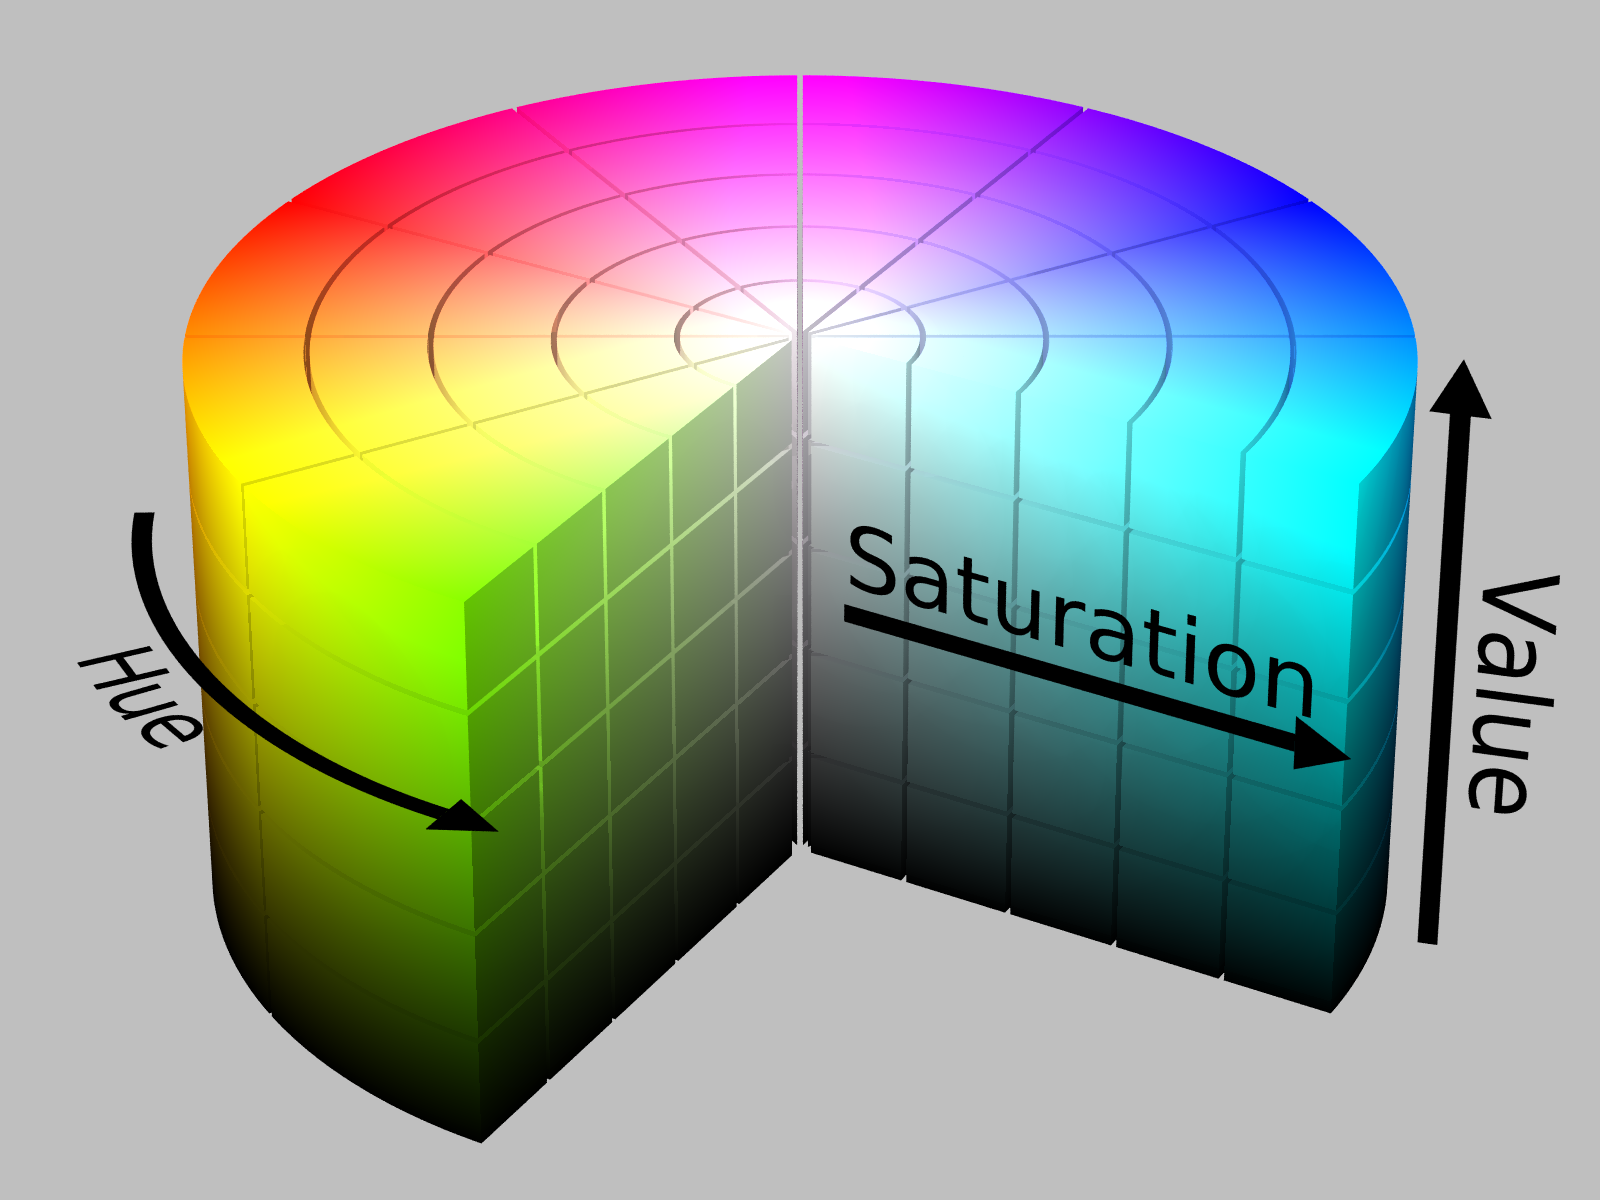
\includegraphics[width=0.5\linewidth]{hsv}

\url{http://en.wikipedia.org/wiki/File:HSV_color_solid_cylinder_alpha_lowgamma.png}
\end{center}


The complex number $z=x+iy$ is converted into its trogonometrical representation $x=r\cdot \cos\phi$ 
and $y=r\cdot \sin\phi$ with $r=\sqrt{x^2+y^2}$. The values $r$ and $\phi$ are now taken as values
for the hsv color model with a constant second value for saturation. $\phi$ is used
for hue. For example: \verb|hsvrgb=phi,1,r|, which gives

\begin{lstlisting}
\DomainColoring[resolution=1000,grfOptions={width=0.49\linewidth},domain={-2,2,-2,2},
   funcName=f10,hsvrgb={phi,1,r}]{}
\hfill
\DomainColoring[resolution=1000,hsvrgb={phi,1,r^2/(1+r^2)},Rmax=2,domain={-2,2,-2,2},
   grfOptions={width=0.49\linewidth}]{cmath.sin(z)*cmath.sin(0.99*z)}
\end{lstlisting}

\noindent
\DomainColoring[resolution=1000,grfOptions={width=0.49\linewidth},domain={-2,2,-2,2},
  funcName=f10,hsvrgb={phi,1,r}]{} % the default
\hfill
\DomainColoring[resolution=1000,hsvrgb={phi,1,r^2/(1+r^2)},Rmax=2,domain={-2,2,-2,2},
   grfOptions={width=0.49\linewidth}]{cmath.sin(z)*cmath.sin(0.99*z)} 

%For $r$ and $\phi$ we have to use $r$ and $phi$.
The optional argument \Lkeyword{hsvrgb} must define three values which can use the arguments
phi and r in any mathematical combination. It must only be compatible to the Lua math conventions,
e.g. \texttt{hsvrgb=\{phi+2,0.5,2/r\}}

\begin{lstlisting}
\DomainColoring[resolution={1000,1000},
   domain={-5,5,-5,5}, grfOptions={width=0.32\linewidth},
   hsvrgb={0.5,r/5,5-r},funcName=f16]{}
\hfill
\DomainColoring[resolution={1000,1000},
   domain={-5,5,-5,5}, grfOptions={width=0.32\linewidth},
   hsvrgb={0.5,5-r,5/r},funcName=f16]{}
\hfill
\DomainColoring[resolution={1000,1000},
   domain={-5,5,-5,5}, grfOptions={width=0.32\linewidth},
   hsvrgb={phi,r/5,5-r},funcName=f16]{}
\end{lstlisting}

\noindent
\DomainColoring[resolution={1000,1000},
   domain={-5,5,-5,5}, grfOptions={width=0.32\linewidth},
   hsvrgb={0.5,r/5,5-r},funcName=f16]{}
\hfill
\DomainColoring[resolution={1000,1000},
   domain={-5,5,-5,5}, grfOptions={width=0.32\linewidth},
   hsvrgb={0.5,5-r,5/r},funcName=f16]{}
\hfill
\DomainColoring[resolution={1000,1000},
   domain={-5,5,-5,5}, grfOptions={width=0.32\linewidth},
   hsvrgb={phi,r/5,5-r},funcName=f16]{}



\subsection{External function definition}
The already existing file \LFile{domaincoloring-functions.lua} collects sone
definitions of complex functions $f(z)$, which can be used from inside \LaTeX\ 
with the optional argument \Lkeyword{funcName}\texttt{<Lua function name>}. 
In this case the mandatory argument
of \Lcs{DomainColoring} has no meaning and can be empty.

\begin{lstlisting}
\DomainColoring[domain={-1.5,1.5,-1.5,1.5},resolution={1001,1001},hsvrgb={phi,1,1/r},
  grfOptions={width=0.49\linewidth},funcName=f12,bgcolor={1,1,1}]{}
\hfill
\DomainColoring[domain={-2.5,1.5,-2,2},resolution={1001,1001},hsvrgb={phi,1,1/r},
  grfOptions={width=0.49\linewidth},funcName=f13,bgcolor={1,1,1}]{}
\end{lstlisting}


\noindent
\DomainColoring[domain={-1.5,1.5,-1.5,1.5},resolution={1001,1001},hsvrgb={phi,1,1/r},
  grfOptions={width=0.49\linewidth},funcName=f12,bgcolor={1,1,1}]{}
\hfill
\DomainColoring[domain={-2.5,1.5,-2,2},resolution={1001,1001},hsvrgb={phi,1,1/r},
  grfOptions={width=0.49\linewidth},funcName=f13,bgcolor={1,1,1}]{}



The contents of the function file of the current version of \LPack{domaincoloring} is::

\lstinputlisting[language={[5.3]Lua},basicstyle=\small\ttfamily]{domaincoloring-functions.lua}



\nocite{*}
\printbibliography

\printindex
\end{document}
